\documentclass[11pt,a4paper,twoside]{tesis}
% SI NO PENSAS IMPRIMIRLO EN FORMATO LIBRO PODES USAR
%\documentclass[11pt,a4paper]{tesis}

\usepackage{graphicx}
\usepackage[utf8]{inputenc}
\usepackage[spanish]{babel}
\usepackage{csquotes}
\usepackage{pifont}
\usepackage[left=3cm,right=3cm,bottom=3.5cm,top=3.5cm]{geometry}
\usepackage[backend=biber,style=numeric]{biblatex} % estilo APA, podés cambiarlo
\addbibresource{tesis.bib} % nombre de tu archivo .bib

% Paquete para glosario
\usepackage[toc, acronym]{glossaries}


% Paquetes para gráficos
\usepackage{tikz}
\usetikzlibrary{arrows.meta, positioning, shapes.multipart, shapes.geometric, shapes, shadows, backgrounds,fit,calc}
%\usetikzlibrary{positioning,shapes,arrows.meta,shadows,backgrounds}

\tikzset{
  block/.style={rectangle, draw, fill=blue!10, rounded corners,
                minimum height=1cm, minimum width=2.8cm, align=center},
  block2/.style={rectangle, draw, fill=red!10, rounded corners,
                minimum height=1cm, minimum width=2.8cm, align=center},
  block3/.style={rectangle, draw, fill=yellow!10, rounded corners,
                minimum height=1cm, minimum width=2.8cm, align=center},
  db/.style={cylinder, draw, fill=green!10, aspect=0.25, shape border rotate=90,
             minimum height=1cm, minimum width=2.5cm, align=center},
  db2/.style={cylinder, draw, fill=red!10, aspect=0.25, shape border rotate=90,
             minimum height=1cm, minimum width=2.5cm, align=center},
%ellipse/.style={ellipse, draw, fill=blue!10, align=center},
  arrow/.style={-{Stealth}, thick},
%  every node/.style={font=\sffamily},
  comp/.style={draw, rounded corners, minimum width=2.8cm, minimum height=1cm, align=center, fill=violet!20, drop shadow},
  webserver/.style={draw, rounded corners, minimum width=2.8cm, minimum height=1cm, align=center, fill=yellow!20, drop shadow},
  appserver/.style={draw, rounded corners, minimum width=2.8cm, minimum height=1cm, align=center, fill=blue!20, drop shadow},
  lb/.style={draw, ellipse, minimum width=2.5cm, minimum height=1.2cm, align=center, fill=green!20, drop shadow},
  server/.style={draw, densely dashed, rounded corners, inner sep=4mm},%, fill=gray!5}
  server2/.style={draw, densely dashed, rounded corners, inner sep=4mm, color=green},%, fill=blackgray!5}
  sharedFS/.style={cylinder, draw, fill=red!10, aspect=0.25, shape border rotate=90,
             minimum height=1cm, minimum width=2.5cm, align=center}, 
}


% Paquete para comentarios en el pdf.
\usepackage{xargs} 
\usepackage[colorinlistoftodos,prependcaption,textsize=tiny]{todonotes}
\newcommandx{\unsure}[2][1=]{\todo[linecolor=red,backgroundcolor=red!25,bordercolor=red,#1]{#2}}
\newcommandx{\change}[2][1=]{\todo[linecolor=blue,backgroundcolor=blue!25,bordercolor=blue,#1]{#2}}

%habilito el glosario
\makeglossaries
\newglossaryentry{LDAP}{
    name=LDAP,
    description= LDAP significa Protocolo Ligero de Acceso a Directorios (Lightweight Directory Access Protocol) y es un protocolo de software que se utiliza para buscar acceder y administrar servicios de directorio a través de una red como bases de datos de información de usuarios cuentas y contraseñas para la autenticación centralizada de aplicaciones y servicios en una organización.,
    plural=LDAP
}

\newglossaryentry{dw_descr}{
    name=data warehouse,
    description= base de datos masiva que se utiliza para realizar análisis de información de negocio para la toma de decisiones,
    plural=Data Warehouses
}

\newglossaryentry{gob}{
    name=gobierno,
    description= descripcion de prueba,
    plural=LDAP
}

\newglossaryentry{af}{
    name=área funcional,
    description=areas de la organización encargadas de actividades no vinculadas a la industria en particular sino también consideradas de soporte de negocio ejemplos pueden ser \gls{rh},
    plural=áreas funcionales.
}

\newglossaryentry{ti}{
    name=IT,
    description=Information Technology,
    plural=IT
}

\newglossaryentry{pm}{
    name=portfolio management,
    description=Metodologías y procesos para poder administrar una cartera de activos,
    plural=portfolio management
}

\newglossaryentry{auto}{
    name=automatización,
    description=Reemplazo de trabajo manual por mecanismos automáticos que eviten la intervención humana.,
    plural=automatizaciones
}

\newglossaryentry{dam}{
    name=decentralized Access Management,
    description=Implementación de procesos sistemas y roles que permite eque la gestión de acceso se realice de forma descentralizada.
    plural=decentralized Access Management
}

\newglossaryentry{gproc}{
    name=global process,
    description=proceso estandard y unificado seguido de por todas las subsidiarias de una compañía global para lograr un objetivo determinado.,
    plural=global processes
}

\newglossaryentry{lux}{
    name=lean UX,
    description = User Experience minimalista,
    plural=lean UXs
}

\newglossaryentry{wapp}{
    name=web application,
    description=Aplicación con arquitectura diseñada para correr en entornos web y ser accedida mediante browsers de internet.,
    plural=web applications
}

\newglossaryentry{webserver}{
    name=web server,
    description=Un servidor web es un sistema (que puede ser tanto hardware como software) que almacena y entrega el contenido de sitios web a los navegadores de los usuarios a través de internet. 
    plural=web servers
}


\newglossaryentry{techstack}{
    name=stack tecnológico,
    description=conjunto de tecnologías utilizadas para implementar una solución desde el software de base tecnologías de base de datos sistema operativo lenguaje de programación librerías.
    plural=stacks tecnológicos
}

\newglossaryentry{loadbalancer}{
    name=load balancer,
    description=Componente de networking especializado para repartir altos volúmenes de pedidos en múltiples servidores.
    plural=load balncers
}

\newglossaryentry{clientserver}{
    name=client server,
    description=Tipo de arquitectura donde existen dos componentes. un cliente (o múltiples) y un servidor que atiende los pedidos de estos clientes los procesa y les devuelve un resultado.
    plural=client server
}

\newglossaryentry{backend}{
    name=back end,
    description=Componente en arquitecturas client server para webapps que se encarga de la persitencia de datos.
    plural=back ends
}

\newglossaryentry{cache}{
    name=cache,
    description=Componente de se utiliza para acelerar el desempeño de aplicaciones que almacena copias locales de datos utilizados frecuentemente para disminuir el tráfico por la red.
    plural=caches
}

\newglossaryentry{faulttolerance}{
    name=fault tolerance,
    description=Tolerancia a fallas: concepto de diseño de incluye puede incluir técnicas de redundancia para que un sistema no deje de funcionar cuando se manfiestan fallas en alguno de sus componentes.
    plural=fault tolerance
}

\newacronym{ldap}{LDAP}{Lightweight Directory Access Protocol}
\newacronym{etl}{ETL}{Extract, Transform and Load}
\newacronym{dw}{DW}{Data Warehouse}
\newacronym{rh}{RR.HH.}{Recursos Humanos}
\newacronym{it}{TI}{Tecnología de la información}
\newacronym{bi}{BI}{Business Intelligence}
\newacronym{kpi}{KPI}{Key Performance Indicator}
\newacronym{ux}{UX}{User Experience}
\newacronym{soa}{SOA}{Service Oriented Architecture}
\newacronym{uat}{UAT}{User Acceptance Test}
\newacronym{dev}{DEV}{Development / Desarrollo}
\newacronym{prd}{PRD}{Production/Producción}
\newacronym{mvc}{MVC}{Model View Controller}
\newacronym{mvp}{MVP}{Minimum Viable Product}
\newacronym{nfs}{NFS}{Network File System}
\newacronym{api}{API}{Application Programming Interface}
\newacronym{rls}{RLS}{Row Level Security}
\newacronym{dbserver}{DB Server}{Database Server}
\newacronym{sso}{SSO}{Single Sign On}
\newacronym{sdlc}{SDLC}{Software Development Lifecycle}
\newacronym{raci}{RACI}{Responsible Accountable Consult Inform}
\newacronym{ttt}{TTT}{Train The Trainers}
\newacronym{cop}{CoP}{Community of Practice}
\newacronym{fte}{ETC}{Empleados de Tiempo Completo}

%\cite{cohesion}.
%\cite{coupling}.
%\cite{webserver}.
%\cite{loadbalancer}.
%\cite{webappserver}.
%\cite{backend}.
%\cite{clientserver}.
%\cite{cache}.
%\cite{faulttolerance}.
%\cite{dbserver}.

\begin{document}

%%%% CARATULA

\def\autor{Pablo S. Casullo}
\def\tituloTesis{Experience Report: \vspace{.2cm} \\ ReportsHub}
\def\runtitulo{Experience Report: ReportsHub}
\def\runtitle{Experience Report: ReportsHub}
\def\director{Diego Garbervetsky}
%\def\codirector{Master Yoda}
\def\lugar{Buenos Aires, 2025}
\newcommand{\HRule}{\rule{\linewidth}{0.2mm}}
%
\thispagestyle{empty}

\begin{center}\leavevmode

\vspace{-2cm}

\begin{tabular}{l}

\includegraphics[width=2.6cm]{logofcen.pdf}
\end{tabular}


{\large \sc Universidad de Buenos Aires

Facultad de Ciencias Exactas y Naturales

Departamento de Computaci\'on}

\vspace{6.0cm}

%\vspace{3.0cm}
%{
%\Large \color{red}
%\begin{tabular}{|p{2cm}cp{2cm}|}
%\hline
%& Pre-Final Version: \today &\\
%\hline
%\end{tabular}
%}
%\vspace{2.5cm}

\begin{huge}
\textbf{\tituloTesis}
\end{huge}

\vspace{2cm}

{\large Tesis de Licenciatura en Ciencias de la Computaci\'on}

\vspace{2cm}

{\Large \autor}

\end{center}

\vfill

{\large

{Director: \director}

\vspace{.2cm}

%{Codirector: \codirector}

\vspace{.2cm}

\lugar
}

\newpage\thispagestyle{empty}


%%%% ABSTRACTS, AGRADECIMIENTOS Y DEDICATORIA
\frontmatter
\pagestyle{empty}
%\begin{center}
%\large \bf \runtitulo
%\end{center}
%\vspace{1cm}
\chapter*{\runtitulo}

\noindent 

En las grandes corporaciones multinacionales coexisten múltiples tecnologías y prácticas de \gls{bi} que abarcan todo el espectro del \gls{techstack}, desde el \gls{dw}, pasando por los procesos de \gls{etl} \cite{inmon1992} hasta herramientas de visualización y análisis. A pesar de los intentos por establecer estándares tecnológicos y de \Gls{gob} \cite{isaca2012}, la descentralización de iniciativas entre áreas funcionales y niveles geográficos genera un ecosistema complejo, heterogéneo y difícil de armonizar. Este escenario plantea importantes desafíos tanto en la integración de soluciones como en la medición de su impacto en el negocio, donde la relación entre adopción e valor resulta poco evidente\cite{davenport2006}. En este contexto, definir \glspl{kpi} de adopción se vuelve crítico para gestionar de manera eficiente el portafolio de soluciones de \gls{bi}, aunque su implementación requiere superar barreras metodológicas y organizacionales. Asimismo, la \gls{ux} se ve afectada por la falta de consistencia en el manejo de los accesos y servicios, lo que refuerza la necesidad de establecer enfoques más integrados y estandarizados en la gestión de estas herramientas.

Estas corporaciones, suelen tener prácticas de definiciones de estándares tecnológicos, que definen herramientas o tecnologías oficiales a ciertos productos y a proveedores, con el fin de simplificar y lograr sinergías tecnológicas entre las herramientas seleccionadas y reducir las combinaciones, según distintos casos de uso\cite{jacobson1986}.

\bigskip

\noindent\textbf{Palabras claves:} \emph{\gls{bi}, \gls{dw}, \Gls{techstack}, \Gls{ux},  \Gls{pm}, \Gls{auto}, \Gls{dam}, \Gls{gproc}, \Gls{gob}.}




\cleardoublepage
%%\begin{center}
%\large \bf \runtitle
%\end{center}
%\vspace{1cm}
\chapter*{\runtitle}

\noindent In large multinational corporations, multiple business intelligence technologies and practices coexist, spanning the entire technology stack, from extraction, transformation, and loading (ETL) processes \cite{inmon1992} to visualization and analytics tools. Despite attempts to establish technological and governance standards \cite{isaca2012}, the decentralization of initiatives across functional areas and geographic levels creates a complex, heterogeneous ecosystem that is difficult to harmonize. This scenario poses significant challenges both in integrating solutions and in measuring their business impact, where the relationship between adoption and impact is often unclear \cite{davenport2006}. In this context, defining adoption metrics becomes critical to coherently managing the business intelligence solutions portfolio, although its implementation requires overcoming methodological and organizational barriers. Likewise, the user experience is affected by the lack of consistency in access and services, reinforcing the need to establish more integrated and standardized approaches in the management of these tools.
These corporations typically have practices for defining technological standards, which establish official tools or technologies for certain products and vendors, with the aim of simplifying and achieving technological synergies among selected tools and reducing combinations according to different use cases \cite{jacobson1986}.

\bigskip

\noindent\textbf{Keywords:} Data Warehouse, Business Intelligence, Portfolio Management, Automation, Distributed Access management, Global Process. % OPCIONAL: comentar si no se quiere

\cleardoublepage
\chapter*{Agradecimientos}

\noindent Lorem ipsum dolor sit amet, consectetur adipiscing elit. Fusce sapien ipsum, aliquet eget convallis at, adipiscing non odio. Donec porttitor tincidunt cursus. In tellus dui, varius sed scelerisque faucibus, sagittis non magna. Vestibulum ante ipsum primis in faucibus orci luctus et ultrices posuere cubilia Curae; Mauris et luctus justo. Class aptent taciti sociosqu ad litora torquent per conubia nostra, per inceptos himenaeos. Mauris sit amet purus massa, sed sodales justo. Mauris id mi sed orci porttitor dictum. Donec vitae mi non leo consectetur tempus vel et sapien. Curabitur enim quam, sollicitudin id iaculis id, congue euismod diam. Sed in eros nec urna lacinia porttitor ut vitae nulla. Ut mattis, erat et laoreet feugiat, lacus urna hendrerit nisi, at tincidunt dui justo at felis. Class aptent taciti sociosqu ad litora torquent per conubia nostra, per inceptos himenaeos. Ut iaculis euismod magna et consequat. Mauris eu augue in ipsum elementum dictum. Sed accumsan, velit vel vehicula dignissim, nibh tellus consequat metus, vel fringilla neque dolor in dolor. Aliquam ac justo ut lectus iaculis pharetra vitae sed turpis. Aliquam pulvinar lorem vel ipsum auctor et hendrerit nisl molestie. Donec id felis nec ante placerat vehicula. Sed lacus risus, aliquet vel facilisis eu, placerat vitae augue.
 % OPCIONAL: comentar si no se quiere

\cleardoublepage
\hfill \textit{A mi persona favorita.}
  % OPCIONAL: comentar si no se quiere

\cleardoublepage
\tableofcontents

\mainmatter
\pagestyle{headings}

%%%% ACA VA EL CONTENIDO DE LA TESIS

\chapter{Motivacion}

\section{Contexto organizacional}
%{\begin{small}%
%\begin{flushright}%
%\it
%There's nothing for me now.
%I want to learn the ways of\\ the Force and become a Jedi like my father. \\
%--Luke Skywalker
%\end{flushright}%
%\end{small}%
%\vspace{.5cm}}

En las grandes corporaciones multinacionales, existen múltiples tecnologías para resolver distintos desafíos de análisis e inteligencia de negocios, a lo largo de todo el stack tecnológico que va desde los sistemas \gls{etl} \cite{inmon1992}, distintos repositorios de almacenamiento para datos estructurados y no estructurados, y herramientas de exploración y explotación de datos que se asocian a la capa de presentación. En esta última coexisten planillas de cálculo (xls) y software específico de visualización para crear reportes y tableros de información, tales como Microstrategy, Cognos, PowerBI, Tableau o Qlik, entre otros.

Estas corporaciones suelen definir estándares tecnológicos que determinan herramientas o proveedores oficiales, con el fin de simplificar y lograr sinergias entre las tecnologías seleccionadas y reducir las combinaciones según distintos casos de uso \cite{jacobson1986}.

Adicionalmente, es común que las iniciativas de inteligencia de negocios estén descentralizadas y distribuidas tanto en áreas funcionales (marketing, ventas, compras, finanzas), como en distintos niveles geográficos, que abarcan desde equipos corporativos hasta instancias globales, regionales y locales.

\section{Situación inicial y limitaciones detectadas}

Este contexto de distribución de recursos en áreas y geografías, combinado con la multiplicidad de herramientas “aprobadas” por dichas corporaciones, genera una combinación de componentes para la creación de distintas soluciones que, aun siguiendo las mejores prácticas de gobernanza tecnológica y de arquitectura \cite{isaca2012}, devienen en un ecosistema complejo, desarmonizado y lleno de particularidades.

Poder establecer el valor real e impacto que estas soluciones tienen en el negocio es un desafío, ya que en muchos casos la relación entre adopción e impacto es indirecta y no trivial \cite{davenport2006}. A su vez, la experiencia de los distintos usuarios varía significativamente: solicitar acceso o encontrar los enlaces de cada herramienta resulta inconsistente, incoherente y dependiente de qué equipo haya desarrollado la solución.

\section{Problemas principales para usuarios y equipos de datos}
\subsection{Gestión de accesos}

La gestión de accesos junto con la aplicación de políticas de seguridad una vez otorgados los mismos, variaban absolutamente y quedaban definidas por el criterio de cada equipo que desarrollaba los contenidos, sin haber coherencia alguna.
Algunos ejemplos de variantes incluyen:

Enviar un email a quien dio las capacitaciones (en caso que las haya habido). Muchas veces la persona encargada de la instrucción o entrenamiento de usuarios era también la encargada de controlar el acceso y otorgarlo. En otros casos, actuaba como intermediario para poder llegar a quien era responsable de otorgar los accesos adecuados.
Solicitar acceso mediante herramientas de tickets a equipos encargados de la operación de dichos tableros/reportes. En equipos de proyecto de tamaños medio o grandes (con un número de integrantes excediendo la decena), es común que haya gente dedicada exclusivamente a tareas operativas, cuyo objetivo es por un lado garantizar la continuidad y máxima disponibilidad de las soluciones como así también en ocasiones se encargan de ejecutar las actividades que habilitan acceso y perfiles de seguridad adecuados a los usuarios.
Solicitar acceso a alguien conocido si puede hacer de nexo para dar con el contacto indicado.

\subsection{Consumo de contenidos}

Para poder consumir o utilizar reportes es fundamental saber de su existencia, conocer su ubicación (normalmente son enlaces dentro de redes internas) y tener acceso a los mismos.
Algunos ejemplos acerca de cómo acceder, pueden incluir:

\begin{enumerate}
    \item Usuarios reciben enlaces de acceso por emails o en documentos de entrenamientos y luego (con suerte) los almacenan como atajos en sus navegadores (con los problemas de tener hardcoded links que luego con el tiempo pueden variar, apuntar a versiones obsoletas de dichos reportes o incluso quedar deprecados conforme algunos reportes son decomisionados).
    \item Páginas de intranet donde se publican los puntos de acceso (muchas veces implementadas como portales de acceso, provistos por las mismas herramientas de visualización).
    \item Usuarios reciben reportes como archivos adjuntos en correos electrónicos.
\end{enumerate}

\subsection{Manejo del portafolio de soluciones de inteligencia de negocios}

Para poder hacer un manejo efectivo de un portafolio de soluciones y de las tecnologías que se utilizan, es necesario poder entender:

¿Qué soluciones hay disponibles y en qué tecnologías están desarrolladas (inventario)?

¿Qué áreas de negocio cubren y quienes son responsables?

¿Qué nivel de adopción tienen?

¿Qué usuarios tienen acceso y no deberían?

¿Qué usuarios necesitan acceso y no tienen?

¿Qué usuarios tienen acceso y no lo usan?

¿Qué usuarios tienen altos nivel de adopción?

¿Qué volumen de pedidos de acceso manejan, según las audiencias objetivo?

¿Hay duplicidad de contenidos, hechos por áreas afines pero sin colaborar?

¿Hay patrones de uso de reportes que tengan correlación con el desempeño de áreas de negocio?

La respuesta a cada una y en particular a todas estas preguntas, en el entorno descripto, es de un esfuerzo que no permite tener información en tiempo y forma ni de modo adecuado, repetible y consistente de manera constante. Poder responder cada pregunta en un contexto tan heterogéneo, implica un nivel de trabajo manual, armonización y alineación de criterios y definiciones que simplemente lo vuelven imposible, en la escala de estas organizaciones.

\newpage
En resumen, los impactos negativos descriptos anteriormente pueden sintetizarse en la siguiente lista: 

\begin{itemize}
\item Falta de un repositorio central y común donde buscar/encontrar y solicitar acceso a los contenidos necesarios genera dificultad para poder dar con los contenidos.
\item Procesos inconsistentes y altamente variables.
\item Falta de transparencia en cuanto a puntos de contactos de reportes.
\item Métodos de aprobación de múltiples pasos y manuales, que dependen de horarios laborales, feriados distribuidos en varias zonas horarios y múltiples geografías.
\item Separación entre nivel de aprobación (hecha por la persona responsable) de un acceso y el nivel de ejecución de dicho acceso (hecha por operadores, una vez que la persona responsable ha definido qué acceso corresponde).
\item Falta de información necesaria para el aprobador, acerca de rol, país, función y otros elementos que ayudan a determinar si un acceso debe o no ser otorgado a un usuario.
\item La ausencia de un repositorio centralizado agrava los problemas de consistencia y coherencia. Esto se traduce en dificultades para asegurar estándares de seguridad homogéneos, en la duplicación de esfuerzos.
\item El estado fragmentado limita la capacidad de contar con indicadores confiables y oportunos para la toma de decisiones de portafolio. 
\item La falta de métricas unificadas de adopción impide evaluar el impacto de las soluciones desarrolladas, dificultando la gestión adecuada del portafolio de inteligencia de negocios.
\end{itemize}


\section{Aporte de la Tesis}
Esta \textit{tesis}, en formato de Experience Report, tiene como objetivo, profundizar en el proceso de desarrollo de una solución que atiende a los desafíos mencionados, detallando desde su concepción en el contexto organizacional, hasta su despliegue y medición del impacto, dentro de una organización de estas características.

Los contenidos a desarrollar incluyen:

\textbf{Definiciones Preliminares:} Conjunto de definiciones básicas que nos introducen en el dominio del problema.

\textbf{Propuesta:} Descripción detallada conceptual de la solución, en función de sus requerimientos funcionales y no funcionales. \cite{zave1979} \cite{yeh1980}

\textbf{Arquitectura:} Descripción de los componentes y sus relaciones como también algunos patrones de diseño aplicados. \cite{yourdon1979} \cite{erl2005} \cite{fowler2003}

\textbf{Desarrollo y Despliegue:} Explicación de la metodología aplicada y entregas iterativas. 

\textbf{Evaluación:} Monitoreo y evaluación de las métricas clave y factores de éxito.

\textbf{Lecciones aprendidas:} Hallazgos y aprendizajes de la experiencia en el proyecto.

\textbf{Conclusiones:} Síntesis final del trabajo, con implicancias finales.

%\unsure { es una prueba de unsure para ver si funciona, está piola}

\chapter{Definiciones Preliminares}

Las definiciones preliminares son aquellas que nos permiten profundizar en los elementos básicos del dominio de nuestro contexto. A continuación se presentan las que aplican a conceptos, roles y elementos clave utilizados a lo largo de este trabajo.

\section{Definiciones de industria y corporaciones multinacionales}
\begin{description}
    \item [KPIs:] Key Performance Indicators (Indicadores clave de desempeño).
\end{description}

\section{Definiciones de inteligencia de negocios}

\begin{description}
    \item [Inteligencia de negocios:] (Business intelligence)
    \item [Data Warehouse:]
\end{description}

\section{Definiciones de diseño y arquitectura de software}
\begin{description}
    \item[Stack tecnológico:] 
    \item [Web App:]
    \item [RLS:]
    \item [LDAP:]
    \item [API:]
    \item [SOA:]
    \item [Cohesión:]
    \item [Acoplamiento:]
    \item [Web Server:]
    \item [Load Balancer:]
    \item [Web Application Server:]
    \item [Back end:]
    \item [Client Server:]
    \item [Caché:]
    \item [Tolerancia a fallas:]
    \item [NFS:]
    \item [Database Server:]
    \item [MVC:] Model View Controller \cite{pope1988}. Patrón de diseño mediante el cual, se separan en tres capas bien definidas, para mayor flexibilidad, mantenibilidad y escalabilidad.
    
\end{description}

\section{Definiciones de metodologías}
    
\begin{description}

\item[Waterfall/Cascada:] Descripción de la Metodología waterfall.
\item[Agile/Agil:] Descripción de la Metodología ágil.
\item[DevOps:] Metodología DevOps.
\item[Unit tests:] Pruebas unitarias.
\item[Integration tests:] Pruebas de integración.
\item[Dev:] Desarrollo. Entorno para desarrollo y pruebas de unidad y de integración.
\item[UAT:] User Acceptance Test. Entorno de pruebas de usuario y validaciones finales antes de hacer pasajes a producción.
\item[Pr:] Production/Producción. Entorno de operaciones productivo.

\end{description}

\section{Definiciones propias del proyecto}

\begin{description}

\item[ReportHub:] Plataforma propuesta para consolidar y armonizar la publicación de reportes y tableros, gestión de accesos y monitoreo de métricas de uso de BI.

\item[Administradores:] Usuarios con privilegios para gestionar contenidos, accesos y usuarios dentro de la plataforma. Se distinguen tres tipos:
    \begin{itemize}
        \item \textbf{Admin Global:} Gestiona unidades geográficas globales y áreas de información a nivel global.
        \item \textbf{Admin Local:} Gestiona áreas de información dentro de su región geográfica asignada.
    \end{itemize}

\item[Creadores de Contenidos:] Usuarios responsables de generar y publicar contenidos dentro de la plataforma.

\item[Consumidores de Contenidos:] Usuarios que acceden y utilizan los contenidos publicados en el portal, pudiendo también marcar favoritos y realizar solicitudes de acceso.

\item[Aprobadores:] Usuarios que evalúan y aprueban solicitudes de acceso a contenidos según la configuración de seguridad definida.

\item[Estructura de contenidos:] Jerarquía de organización de contenidos en dos niveles:
    \begin{enumerate}
        \item \textbf{Nivel 1:} Unidades geográficas (Global, Europa, América, Asia, África y países correspondientes).
        \item \textbf{Nivel 2:} Áreas de información (temáticas específicas, únicas dentro de cada región).
    \end{enumerate}

\item[Metadatos de Contenido:] Información asociada a cada contenido publicado, incluyendo:
    \begin{itemize}
        \item Título
        \item Descripción
        \item Imagen miniatura
        \item Tipo de contenido (archivo o URL)
        \item Segmentos de usuarios y objetivos de frecuencia de uso
        \item Aprobadores
        \item Configuración de provisión de acceso
    \end{itemize}


\end{description}

\chapter{Propuesta}
\section{Visión y objetivos del proyecto}

Por todo lo anteriormente descrito, es que surge este proyecto, impulsando un espacio de consolidación y armonización de publicación, gestión de accesos y monitoreo de métricas de uso para la adecuada gestión del portafolio de BI. Asimismo, unificar el acceso y ofrecer una experiencia homogénea y consistente, independiente de la tecnología de implementación, se presenta como una oportunidad para mejorar tanto la eficiencia de los equipos de datos como la satisfacción de los usuarios finales.

De la complejidad de estas problemáticas surgió la necesidad de lograr una solución que permita:

Concentrar en un solo lugar la oferta de reportes/tableros ofrecida por los distintos equipos.
Permitir a los equipos que publican estos elementos, realizar una gestión de sus usuarios, incluyendo la asignación de roles si aplican restricciones de visibilidad de datos.
Establecer objetivos de adopción y medirlos de modo consistente, de manera totalmente independiente a la tecnología de implementación que se haya utilizado.
Darle a los potenciales usuarios una experiencia homogénea y consistente, de modo agnóstico a las tecnologías utilizadas mediante técnicas de ingeniería de software.
A los usuarios, almacenar atajos o accesos directos “resilientes” que resistan cambios de URLs de reportes y a la vez conserven atributos de seguridad para que compartiendo los enlaces la seguridad se mantenga.

\section{Principios de diseño de ReportHub}

El diseño de la solución se basó en un conjunto de principios arquitectónicos que aseguraron no solo la cobertura de las necesidades funcionales del momento, sino también la capacidad de evolucionar en el tiempo. Estos principios tuvieron como propósito garantizar que la plataforma fuera escalable, permitiendo crecer en volumen de usuarios, contenidos y procesos sin comprometer el rendimiento. A su vez, aseguraron un mantenimiento eficiente, reduciendo la complejidad técnica y posibilitando la incorporación de nuevas funcionalidades de forma ágil y con bajo costo operativo.
Otro eje fundamental fue la facilidad de uso, que permitió que cada rol interactuara con la solución de manera simple, intuitiva y orientada a sus tareas principales, evitando barreras de adopción. Asimismo, se estableció un marco que permitió cumplir con las normas internas de auditoría, control de calidad y gobierno de la información, garantizando la trazabilidad y responsabilidad en cada acción ejecutada dentro del sistema.
Finalmente, los principios incorporaron las mejores prácticas en seguridad y estándares internacionales, asegurando la protección de datos, la correcta gestión de accesos y la interoperabilidad con diferentes tecnologías, lo que fortaleció la resiliencia y confiabilidad de la solución en contextos de negocio dinámicos y regulados.

La solución debe cumplir con los siguientes principios de diseño:

\subsection{\Gls{wapp}}
\label{principios:webapp}
Será una aplicación web, que contará con una elementos de presentación el el browser, una capa de lógica de negocio en un servidor y se apoyará en una base de datos relacional para almacenar la información y meta información necesaria para la configuración, uso y auditoría de actividades.

\subsection{\gls{lux} minimalista y defensiva}
\label{principios:leanUx}
Experiencia de usuario simple e intuitiva para cada uno de los roles en que los usuarios operen la solución, ya que un mismo usuario, puede tener contenidos para publicar, ser administrador del sistema y eventualmente consumidor de contenidos publicados por otros usuarios:
\begin{itemize}
\item \textit{Administradores, roles:} “Admin Global / Admin Local”.
\item \textit{Creadores de Contenidos, rol:} “Creador”.
\item \textit{Consumidores de contenidos, rol:} “Consumidor”.
\end{itemize}

La interfaz, debe evitar que el usuario cargue información inválida mediante reglas de negocio intuitivas y ya incorporadas a la navegación y cuando esto nos sea posible, validará la información que el usuario ingrese y proveerá feedback inmediato en el momento de las interacciones para poder corregir problemas.

\subsection{Tener una \Gls{soa}}
\label{principios:soa}
Ser agnóstico de las tecnologías en las que se han producido los contenidos que se publicarán minimizando el acoplamiento técnico y a la vez funcionando con una alta cohesión. Este punto permite garantizar la “interoperabilidad" con diferentes tecnologías y a la vez el soporte de procesos comunes, sin estar condicionados por las tecnologías de implementación.

\subsection{Descentrado y Escalable}
\label{principios:federado}
Permitir la descentralización de la gestión de contenidos, accesos y configuraciones de modo de poder asignar en distintos niveles y equipos organizacionales las facultades para el auto servicio de sus contenidos. Esto evita los cuellos de botella de estructuras centralizadas y fomenta que se tomen las decisiones adecuadas en cada lugar adecuado de la organización, siguiendo procesos consistentes garantizados por el sistema.

\subsection{Auditable}
\label{princpipios:auditable}
Cada acción debe ser auditable, para poder cumplir con normas internas de auditorías de calidad de procesos y responsabilidad, en particular a la hora de administrar usuarios y accesos.

\section{Casos de uso principales}
Los principales casos de uso, tienen como objetivo detallar en un nivel conceptual, las funcionalidades básicas y escenarios que iba a soportar el sistema. 

\subsection{Creación de estructuras geográficas para organizar los contenidos (Admin Global).}
Los contenidos del sistema debían estar organizados en una jerarquía de dos niveles. El primer nivel, compuesto de unidades geográficas, tenía como objetivo agrupar por geografía y a su vez, poder otorgar niveles de administración descentralizados a distintos Admins de geografías para administrar áreas de información. Se utilizan como valores válidos, los correspondientes a las distintas unidades geográficas:
	-Global
	-Europa
	-America
	-Asia
	-Africa
	y luego países
	Todos estarán agrupados en un mismo nivel.

\subsection{Creación de áreas de información para organizar los contenidos(Admin Global/Local).}

El segundo nivel de organización son áreas de información y permiten una agrupación lógica de los contenidos en función de las temáticas que cubren, como por ejemplo finanzas, marketing, ventas, etc. No existe un listado predefinido de qué áreas de información existen a nivel local y pueden ser creadas libremente por los administradores a nivel geográfico. La única restricción: los nombres de las áreas en una región geográfica deben ser únicos.


Por ejemplo:

\begin{itemize}
\item Global
    \begin{itemize}
        \item Marketing
        \item Cumplimiento
        \item Ventas
        \item Finanzas
        \item Recursos Humanos, etc.
    \end{itemize}
	\item America
		\begin{itemize}
		    \item Marketing
            \item Legales, etc.
        \end{itemize}
	\item Argentina
        \begin{itemize}
            \item Fuerza de Ventas
            \item Finanzas
            \item Oportunidades, etc.	
        \end{itemize}
\end{itemize}

\subsection{Creación y administración de Usuarios.}

La “creación” y administración de usuarios, consiste en poder registrar usuarios que ya son parte del directorio corporativo como usuarios de este sistema y asignarles roles de Admins globales, locales, de áreas de información y/o eventualmente como consumidores. Del directorio corporativo se importan los siguientes datos: handle de usuario de la compañía, nombre completo, dirección de correo electrónico.

	Es importante aclarar que un Admin tiene la capacidad de crear secciones, contenidos y manejar usuarios, pero no necesariamente tiene acceso a los mismos contenidos que publica, ya que son aspectos guiados por diferentes criterios de seguridad y las personas responsables de los contenidos son quienes deben aprobar los accesos y decidir quienes tienen acceso.
		La forma en la que los permisos serán asignados de acuerdo a los roles se detalla en la tabla \ref{tab:funcxrol}.

        
        Todos los usuarios pueden asignar a otros usuarios  las siguientes reglas de la tabla \ref{tab:asignaciones}:

\begin{table}
    \centering
    \begin{tabular}{|c|c|c|c|c|}\hline
         Función/rol&  Admin global&  Admin local&  Creador& Aprobador\\\hline
         Crear áreas globales&  \ding{51}&  &  & \\\hline
         Crear áreas locales& \ding{51}&  \ding{51}&  & \\\hline
         Crear contenidos&  \ding{51}&  \ding{51}&  \ding{51}& \\\hline
         Administrar usuarios&  \ding{51}&  \ding{51}&  \ding{51}& \ding{51}\\\hline
         Asignar Roles $^1$&  \ding{51}&  \ding{51}&  \ding{51}& \ding{51}\\\hline
         Aprobar accesos&  &  &  \ding{51}& \ding{51}\\ \hline
    \end{tabular}
    \caption{Funciones por rol (\ding{51})}
    \label{tab:funcxrol}
\end{table}



\begin{table}

    \centering
    \begin{tabular}{|c|c|c|c|c|}\hline
         Rol / puede asignar&  Admin global&  Admin local&  Creador& Aprobador\\\hline
         Admin global&  \ding{51} &  \ding{51}&  \ding{51}& \ding{51}\\\hline
         Admin local&  &  \ding{51}&  \ding{51}& \ding{51}\\\hline
         Creador&  &  &  \ding{51}& \ding{51}\\\hline
         Aprobador&  &  &  & \ding{51}\\ \hline
    \end{tabular}
    \caption{Asignaciones de roles válidas (\ding{51})}
    \label{tab:asignaciones}
\end{table}

Estos mecanismos designados, también aplican a la hora de modificar los privilegios de un usuario. En caso de que un usuario vaya a ser desafectado del sistema, debe haber siempre un usuario alternativo como administrador global/local o creador de área de información o contenido. Si en algún momento algún usuario deja de pertenecer a la compañía, y algún área quedara sin administradores, entonces el sistema asignará automáticamente a cargo de los elementos del portal “huérfanos” a quienes sean los responsables inmediatos superiores dentro del mismo, siguiendo la lógica de Aprobador - Creador - Admin Local y Admin Global en última instancia. Para Admins globales debe haber siempre al menos 2 y es parte de la configuración inicial del sistema.

\subsection{Publicación de contenidos (Creador/Admin).}

La publicación de contenidos se hará de modo que cada pieza de contenido estará representada por los siguientes metadatos obligatorios:

\begin{itemize}
\item Título: Un texto denomina al contenido.
\item Descripción: Texto que da una breve descripción de lo que el contenido ilustra o representa.
\item Imagen miniatura: una imagen que representa el contenido, pudiendo ser un logo, un pequeño screenshot o cualquier elemento visual que permita reconocer al contenido publicado.
\item Tipo de Contenido: Los contenidos pueden ser de dos tipos, o bien archivos cargables o bien URLs a elementos que residan dentro de la intranet.
\item Segmentos de usuarios: Debe haber al menos 1 segmento de usuario (segmento por defecto llamado usuarios generales) y se le deben asignar objetivos de frecuencia de uso, en función de una cantidad de veces por unidades de tiempo. 
    Cantidad: Un número natural mayor a cero.
	Frecuencia: deberá ser algún valor de esta lista: “diario, semanal, mensual, trimestral, semestral, anual”

	De este modo, la idea es poder establecer los objetivos de adopción según perfiles de usuario y cómo se espera que estos utilicen los contenidos para poder ser eficientes en sus procesos de negocio.

\item Aprobadores: puede agregarse el listado de aprobadores y por defecto quien crea podrá aprobar acceso.

\item Selección del modo de provisión de acceso:
    \begin{itemize}
    \item En caso que el tipo de Contenido sea un archivo, se aplica la lógica por defecto de acceso directo.
	\item En caso de que el tipo de Contenido sea un enlace a un reporte en otra tecnología, se opta entre dos modelos:
    \begin{enumerate}
        \item Un modelo de control de acceso integrado a un sistema de tickets, donde se debe especificar dentro de ese sistema qué grupo es el encargado de recibir el ticket y se configuran parámetros con los que se creará el ticket, según sean requeridos:
	       \begin{itemize}
	       \item Nombre del reporte al que se pide acceso.
	       \item Nombre de quien solicita el acceso. 
		   \item Handle de usuario.
		   \item Dirección de email.
		   \item Puesto en la compañía.
		   \item País de localización de quien lo pide.
           \end{itemize}
	    \item Si el reporte tiene un modelo de acceso basado en listas de distribución del directorio corporativo, entonces deben especificarse dichas listas y quedarán asociadas al contenido (y se pueden asociar a segmentos de usuarios).
        \end{enumerate}
	\item Si tiene seguridad basada en roles dentro del reporte y de ser así, se definen dos mecanismos posibles:
        \begin{enumerate}
            \item Listas de distribución especificas del directorio corporativo. En este caso se define qué listas del directorio corporativo están asociadas a este contenido, para que el aprobador pueda utilizarlas en el momento de la aprobación.
		    \item Esquema propio de cada contenido con perfiles/roles particulares. En este caso, deben especificarse los end points y credenciales para poder integrar la administración.
        \end{enumerate}
    \end{itemize}
\end{itemize}

\subsection{Descubrimiento y navegación en el catálogo (Consumidor).}

El portal tiene dos modos de operación. Un primer modo predeterminado, que permite utilizar los contenidos asignados, disponibles y ordenados según las unidades geográficas y áreas de información.
	También hay una sección de “Favoritos” que contiene aquellos contenidos elegidos por el usuario como favoritos, que normalmente simplifican el acceso a los que son de uso frecuente.
	Esta la posibilidad de buscar contenidos por textos relacionados a los metadatos definidos en el caso de uso 4.
	El segundo modo, es el modo “catálogo”, donde el usuario consumidor tendrá la posibilidad de ver por unidades geográficas y áreas de información disponibles pero a los que no tiene acceso. Cada elemento podrá ser agregado a un “carrito de compras”, y una vez terminada la selección de los elementos para solicitar acceso, se podrá hacer un pedido formal de acceso. También está la posibilidad de agregar un texto como solicitud, explicando para cada elemento (o de forma colectiva) por qué la persona necesita acceso para los elementos. Cuando el usuario completa la acción de pedir acceso a los elementos del carrito de compras, se dispararán los procesos de aprobación, otorgamiento de accesos y notificación según se hayan definido en cada elemento.


\subsection{Circuito de Aprobaciones (Creador/Admin).}

En el circuito de aprobaciones, quienes son aprobadores recibirán una notificación por email y también tendrán un ícono en el portal que les indicará que tienen “tareas pendientes”. Tanto el email como el ícono, lleva a los aprobadores a la interfaz que les permite evaluar los pedidos en función de las solicitudes que recibieron y poder aprobarlos o rechazarlos de manera general o particular. En caso de rechazo de la solicitud, deben colocar el motivo y en ambos (tanto positivo como negativo) casos el resultado del proceso será informado al usuario solicitante, tanto por email, como una notificación en el portal.
	Adicionalmente, si el contenido al que se solicita acceso, está cargado en el portal, el acceso se otorga de modo directo.
	En caso de que el contenido publicado tenga asociada seguridad manejada por listas de distribución, se hará la asociación en ese momento y si además tiene habilitada la configuración de administración de perfiles de aplicación, se asignarán en el momento.
	Si por último, el contenido publicado, está implementado y operado bajo un modelo de soporte basado en tickets, con la información configurada en el momento de la creación del contenido en el portal, se generará un ticket mediante el equipo correspondiente, adjuntando la información necesaria para el alta y la aprobación del aprobador para que el equipo de mantenimiento tenga el respaldo necesario para poder documentar y accionar el pedido, de acuerdo a las normas de cumplimiento de la empresa. En este caso, la notificación que recibirá el usuario que solicitó acceso tiene un texto que le informa que su pedido fue aprobado y se creó el ticket nro XXX en su nombre, para que pueda darle seguimiento con el equipo de operaciones.


\subsection{Navegación, acceso al portal y a reportes y monitoreo de estadísticas.}

Las acciones de navegación dentro del portal tienen como objetivo poder recorrer los contenidos y accederlos. Para acceder un contenido, bastará con clickear con el mouse sobre la el ícono que lo representa en el catálogo y esto desplegará un nuevo Frame del navegador de internet que será una dirección enmascarada al elemento en cuestión. Esto permitirá que el enlace se pueda guardar como acceso directo y a la vez compartir por el usuario con otras personas, sin exponer el link original y preservando el control de acceso primario. El efecto deseado es agregar un nivel de indirección de modo tal que al guardar el link como acceso directo, quienes publican los contenidos puedan modificar el link interno de acceso sin afectar los enlaces del portal.
	Finalmente, todas las acciones de búsqueda, navegación, gestión de usuarios y de accesos, serán registradas en una bitácora de eventos de modo tal de generar un historial de las transacciones ocurridas, para poder luego poder optimizar el funcionamiento del sitio, aplicar auditorías de cumplimento necesarias y a la vez obtener métricas que permitan medir los criterios de éxito del Portal.	
\section{Alcance inicial y entregables previstos}
El alcance inicial comenzó con la implementación de los casos de uso para los roles de Administrador Global, Creador y Consumidor de contenidos. En una segunda fase se decidió incorporar al perfil de administrador Local para poder agregar una capa intermedia de administración que permita descentralizar y federar el gobierno de los contenidos de modo más eficiente.
Se priorizó también la publicación de contenido global en una primera instancia y luego en etapas sucesivas, luego de la implementación del rol local, se comenzó a expandir a otras unidades geográficas con el abordaje a los equipos locales de múltiples áreas.

\section{Definición de KPIs y métricas de éxito}

Para poder medir el avance y el éxito del proyecto se identificaron métricas de varios tipos:

\begin{itemize}
    \item \textit{Experiencia de usuario}:
	La primer métrica que se definió está asociada al tiempo de respuesta del portal durante las interacciones y en principio, lo que se buscó es que cada interacción, dure entre 300 y 500 milisegundos (sin incorporar el tiempo de latencia de red). Es decir que cada vez que el usuario disparaba una acción sobre el portal, el tiempo de respuesta combinado, desde que enviaba el estímulo hasta que recibía la respuesta completa (o el indicio de respuesta) no debía ser mayor a 1000 milisegundos. Cuando hablamos del indicio de respuesta, nos referimos a que a veces, por volumen de información que debe viajar desde el servidor de base de datos y web hasta el browser del usuario, simplemente no es posible, pero sí se puede comenzar a renderizar parcialmente o dar alguna indicación visual de que su solicitud fue hecha y que está en proceso de ser resuelta.

    \item \textit{Adopción}: Para poder medir la adopción efectiva de la herramienta se estableció como métrica la cantidad de piezas de contenido creadas, cantidad de usuarios creadores, cantidad de usuarios asignados y finalmente actividad asociada según los tipos de transacciones definidos en los casos de uso.

    \item \textit{Ahorros de tiempo y recursos y minimización de errores}:
Para poder hacer una medición de estos elementos se decidió hacer seguimiento de cantidad de tickets generados para gestión de accesos a grupos de soporte. Cantidad de accesos asignados mediante listas de distribución.
\end{itemize}
\chapter{Arquitectura}
\section{Principios de diseño}

Para poder cumplir adecuadamente con los requerimientos funcionales (descriptos anteriormente en los casos de uso Sec. \ref{usecases:main}), como así también de los no funcionales, se decidió implementar diferentes principios de diseño.


A continuación, un detalle de qué principios de diseño se eligieron para dar adecuado soporte.

\begin{table} 
    \centering
    \begin{tabular}{|c|c|}\hline
         Caso de Uso&  Principio de diseño\\\hline
         \ref{usecases:geolevel1}-Gestión de áreas geográficas&  descentralizado y escalable \ref{principios:federado}\\\hline
         \ref{usecases:geolevel2}-Gestión de áreas de información&  descentralizado y escalable \ref{principios:federado}\\\hline
         \ref{usecases:useradmin}-Gestión de usuarios&  descentralizado y escalable \ref{principios:federado}\\\hline
         \ref{usecases:contentadmin}-Gestión de contenidos&  descentralizado y escalable \ref{principios:federado}\\\hline
         \ref{usecases:browse}-Navegación del catálogo y solicitud de acceso&  webapp \ref{principios:webapp} y lean UX\ref{principios:leanUx}\\\hline             
         \ref{usecases:accessmgmnt}-Gestión de accesos y permisos&  descentralizado y escalable \ref{principios:federado}\\\hline 
         \ref{usecases:contentaccess}-Navegacion y acceso a los contenidos&  webapp \ref{principios:webapp} y lean UX \ref{principios:leanUx}\\\hline          
         \ref{usecases:logging}-Logs de actividades y monitoreo de estadísticas& auditable \ref{princpipios:auditable}\\\hline          
    \end{tabular}
    \caption{Mapeo de Casos de uso a principios de diseño}
    \label{tab:usecasesxdesignprinciples}
\end{table}

Para poder responder a diseño escalable y descentralizado, se seleccionó una arquitectura de \emph{\Gls{wapp}}, ya que el encarar el proyecto con este enfoque, en lugar de una arquitectura de cliente servidor tradicional con un cliente compilado, ejecutable e instalado en las máquinas clientes y el código del servidor corriendo en un server, permitió aprovechar el mantenimiento y escalabilidad propias de las arquitecturas de las aplicaciones web. 

En escencia, siguen siendo cliente servidor, con la diferencia de que el código que se ejecuta en el cliente se descarga en el código web al que se accede desde el browswer de internet, de modo que al mantenimiento y el control de versiones, actualizaciones y mejoras se da de modo automático\footnote{En ciertos casos, es posible que haya código descargado en cachés locales, pero pueden invalidarse y actualizarse fácilmente como parte de las actualizaciones.} en cada máquina cliente.


Adicionalmente, con un diseño de despliegue físico adecuado, se puede también escalar horizontalmente sin mayores esfuerzos y aumentar la tolerancia a fallas.


En el caso puntual de esta aplicación, se diseñaron dos configuraciones: una para entornos de desarrollo y pruebas y luego una para un entorno productivo, donde se tolera una carga de usuarios real y debe maximizarse la tolerancia a fallas, donde se agrega un tercer servidor web/de aplicaciones.

\newpage 

Finalmente y de acuerdo a los estándares tecnológicos de este proyecto, se utilizó el siguiente stack tecnológico:

    \begin{itemize}
        \item Loadbalancer de F5
        \item Webserver: Apache
        \item Application server: Tomcat (Java)
        \item RDBMS: Oracle
        \item sistema operativo de servers: RH Linux
    \end{itemize}

A continuación, describimos el diagrama de despliegue físico que permitió implementar la arquitectura de webapp, con máxima tolerancia a fallas en sus componentes de mayor demanda con escalabilidad horizontal.

\begin{figure} [h!]
    \centering
    \begin{tikzpicture} [node distance=1.8cm and 2.5cm]
 % Client
    \node[comp] (client) {Browser};
 % Load Balancer
    \node[lb, below=1cm of client] (f5) {LB};
    \node[server, fit=(f5)] (lbsrv) {};
    % Apache / Tomcat pairs
    \node[webserver, below left=1.2cm and 4cm of f5] (apache1) {Apache};
    \node[appserver, right=0.5cm of apache1] (tomcat1) {Tomcat};
    \node[server, fit=(apache1) (tomcat1)] (srv1) {};
    \node[webserver, below right=3.5cm and -4cm of f5] (apache2) {Apache};
%    \node[appserver, below=0.6cm of apache2] (tomcat2) {Tomcat};
    \node[appserver, right=0.5cm of apache2] (tomcat2) {Tomcat};
    \node[server, fit=(apache2) (tomcat2)] (srv2) {};
    \node[webserver, below right=1.2cm and 1cm of f5] (apache3) {Apache};
    \node[appserver, right=0.5cm of apache3] (tomcat3) {Tomcat};
    \node[server2, fit=(apache3) (tomcat3)] (srv3) {};

    %Shared FS
    \node[sharedFS, below =5cm of apache1] (shaFS) {NFS};    
    \node[server, fit=(shaFS)] (srvSharedFS) {};
    

    % Database
    \node[db, below=5cm of tomcat3] (db) {Oracle\\Database};
    \node[server, fit=(db)] (dbsrv) {};
     % Arrows
    \draw[-{Stealth[length=8pt]}] (client) -- (f5);
    \draw[-{Stealth[length=8pt]}] (f5.west) -| (srv1);
    \draw[-{Stealth[length=8pt]}] (f5.south) -- (srv2);
    \draw[-{Stealth[length=8pt]}] (f5.east) -| (srv3);
    \draw[-{Stealth[length=8pt]}] (apache1) -- (tomcat1);
    \draw[-{Stealth[length=8pt]}] (apache2) -- (tomcat2);
    \draw[-{Stealth[length=8pt]}] (apache3) -- (tomcat3);
    \draw[-{Stealth[length=8pt]}] (tomcat1) -- (apache1);
    \draw[-{Stealth[length=8pt]}] (tomcat2) -- (apache2);
    \draw[-{Stealth[length=8pt]}] (tomcat3) -- (apache3);
    \draw[-{Stealth[length=8pt]}] (tomcat1) |- (db.west);
    \draw[-{Stealth[length=8pt]}] (tomcat2.east) -| (db.north);
    \draw[-{Stealth[length=8pt]}] (tomcat3) -- (db.north);   
    \draw[-{Stealth[length=8pt,color=red]}, draw=red] (apache1.south) -| (shaFS.north);
    \draw[-{Stealth[length=8pt,color=red]}, draw=red] (apache2.south) |- (shaFS.east);
    \draw[-{Stealth[length=8pt,color=red]}, draw=red] (apache3.south) |- (shaFS.east);   
    
  % --- LEYENDA ---
  \matrix [draw, below =10cm of f5, column sep=0.5cm, row sep=0.3cm, nodes={anchor=west}]
  {
    \node[comp, scale=0.5] {}; & \node {Componentes}; &
    \node[lb, scale=0.5] {}; & \node {Load Balancer}; \\
    \node[server, scale=0.7] {}; & \node {Unix Server DEV+UAT+Prd}; &
    \node[server2, scale=0.7] {}; & \node {Unix Server +Prd}; \\
    \node[webserver, scale=0.5] {}; & \node {Web Server}; &
    \node[appserver, scale=0.5] {}; & \node {App Server}; \\
    \node[db, scale=0.6] {};    & \node {Bases de datos de proyectos}; &
    \node[sharedFS, scale=0.6] {};    & \node {Shared FS}; \\
  };    

\end{tikzpicture}
    \caption{Componentes de la arquitectura de la webapp - Diagrama de despliegue físico}
    \label{fig:arq_webapp} 
\end{figure}

\newpage

\begin{enumerate}

    \item \Gls{lux} (\ref{principios:leanUx})

    En el caso del diseño de la interfaz de usuario, no condiciona la arquitectura en sí de la aplicación, aunque influye en la selección de qué tecnologías se utilizarán para implementar las interacciones y los elementos de visualización. La interfaz de usuario, es el sistema de comunicación que tiene el producto de software para brindarle información sobre el estado del sistema, los contenidos y el resultado de las operaciones que el usuario realice con el mismo. 
    
    \item Tener una \gls{soa} (\ref{principios:soa})

    En este caso particular, se buscó implementar una arquitectura orientada a servicios, para la capa de negocio, de modo que pueda hacerse una separación, escalable de ser necesaria de ciertos servicios críticos y de alta demanda. de este modo, se puede seguir escalando la capacidad de la aplicación, en funcion de ciertas operaciones de alta demanda y críticas para brindar los servicios del portal. En otros casos, ciertos servicios se definieron como elementos reusables que pueden ser parte de un ecosistema más grande de aplciaciones y que tenía sentido independizar del bloque inicial de código, somo proyectos "hijos".
    
    \item Descentralizado y escalable (\ref{principios:federado})
    
    La posibilidad de descentralización, tiene que ver con poder distribuir tareas según responsabilidades de ciertos usuarios, en vez de tener un equipo centralizado de gente que opere y administre los contenidos y los manejos de accesos del portal. Esto implica que el volumen de usuarios con la capacidad de ejercer múltiples roles aumenta, en prácticamente un orden de magnitud, de 10x a 100x.
    
    La escalabilidad, se vuelve entonces un aspecto escencial para poder sostener un buen desempeño, desde el punto de vista de la performance y la experiencia de usuario, sin poner en riesgo la estabilidad del sistema. Para dicho fin, la arquitectura de \ref{fig:arq_webapp}, mencionada anteriormente se vuelve clave.
    
    \item Auditable (\ref{princpipios:auditable})
    explicar toda la lógica de auditoría en función de qué transacciones que hayan identificar como auditables y luego empezar a desarrollar cada uno, los temas de metadata que deben registrarse. en un log de auditoría se registra:

    \begin{itemize}
        \item userid: identificador unico del usuario que inicia la transacción.
        \item timestamp (formato de timestamp que representa el instante de tiempo en el que se hizo la transacción con nivel de granularidad de milisegundo).
        \item operación descripción de la operación que se realiza.
        \item campos afectados (con valores anteriores y nuevos en caso de actualizaciones).
        \item id de transacción (para el caso de que haya multiples operaciones en una transacción).
        \item duracion (en milisegundos).
        
    \end{itemize}

    Con toda esta metainformación, es posible obtener una vitácora de las transacciones ocurridas y poder realizar auditorías y análisis varios, tanto para evaluar estadísticas del sistema como así también patrones de uso y performance.
    
\end{enumerate}


\section{Arquitectura}
\section{Componentes principales}

Para avanzar con la implementación de la solución, se decidió implementar un patrón de \gls{mvc}. Dicho enfoque, permite separar claramente en capas lógicas la presentación e interfaz, la lógica de negocio y el modelo de datos, que se alinean muy bien con la arquitectura de webapp.

El mapeo del modelo MVC a la arquitectura de webapp fue hecha del siguiente modo:

Modelo (Model):

En el contexto de una webapp, el modelo representa la parte de la aplicación que maneja los datos y la lógica de negocio. Incluye las clases y objetos que interactúan con la base de datos para almacenar, recuperar y manipular datos.
El modelo se comunica directamente con el motor de bases de datos (RDBMS, Oracle, en este caso) para ejecutar consultas y obtener resultados.
En esta arquitectura de múltiples servidores, el modelo está distribuido, con diferentes instancias de aplicación (Tomcat) accediendo a la misma base de datos compartida a través de un sistema de archivos compartido (NFS).

Vista (View):

La vista es la parte de la aplicación que el usuario interactúa directamente. En una webapp, es la interfaz de usuario presentada en el navegador del usuario.
Las vistas se generan a partir del modelo y son dinámicas, adaptándose a los datos que el modelo proporciona. Las vistas pueden ser renderizadas en el servidor (Tomcat) y/o en el cliente (navegador).
En este caso, las vistas son gestionadas por el servidor web (Apache), que sirve archivos estáticos (HTML, CSS, JavaScript albergados en el NFS) y delega las solicitudes dinámicas al servidor de aplicaciones (Tomcat).

Controlador (Controller):

El controlador es el intermediario entre la vista y el modelo. Es responsable de manejar las solicitudes del usuario, interpretar las acciones y actualizar la vista y/o el modelo en consecuencia.
Aquí, el controlador se encarga de procesar las solicitudes HTTP, extraer los datos de la solicitud, invocar el código de negocio del modelo y devolver una vista actualizada al cliente.
El controlador está implementado en el servidor de aplicaciones, donde maneja las interacciones con el usuario y coordina el flujo de datos entre la vista y el modelo.

A continuación, una breve explicación de cómo el \gls{mvc} se mapeó a esta arquitectura de \Gls{wapp}:

Los componentes se distribuyen a lo largo de los diferentes niveles de la stack tecnológico:

\begin{itemize}
    \item El servidor web (Apache) actúa como el punto de entrada para las solicitudes y atendiendo las solicitudes estáticas y delegando las dinámicas a los componentes tomcats.
    \item El servidor de aplicaciones (Tomcat) ejecuta el controlador y el modelo, procesando las solicitudes y generando las vistas.
    \item El sistema de archivos compartido proporciona el soporte al contenido estático que comparten las instancias de Apache y de Tomcats.
    \item La base de datos (Oracle) proporciona almacenamiento persistente para los datos generados, mantenidos y accedidos por el modelo.
\end{itemize}

A su vez, también, dentro del modelo, se identificaron los siguientes componentes lógicos que permitieron distribuir las actividades de desarrollo y mantener a la vez una estructura modular, de muy alta cohesión y bajo acomplamiento.

\begin{enumerate}
    \item \textbf{ReportsHub}:
        Codigo que contiene la lógica de negocios y la capa de presentación que se sirve a los browsers con los que se accede.

    \item \textbf{User Admin API}: Módulo de interacción con el directorio LDAP, que permite al portal ejecutar operaciones básicas de gestion de usuarios y de listas de distribución y grupos de seguridad.
        
    \item \textbf{RLS API}: Módulo que implementa de manera genérica y universal, la gestión de perfiles de usuarios con el \gls{rls} que se utilice. Este módulo es de uso opcional y depende de un proyecto tiene implementado \gls{rls} o no.
    
        el conjunto de servicios implementados para dicho módulo es el siguiente:
        \begin{enumerate}
            \item **GET\_ROLES**: devuelve una lista de roles de proyecto.
            \item **GET\_USER\_ROLES**: devuelve el rol asociado a un usuario específico - usando un UserID.
            \item **ADD\_USER\_ROLES**: agrega o actualiza un rol a un usuario específico.
            \item **ADD\_USER\_W\_FULL\_NAME\_ROLES**: agrega un rol a un usuario específico enviando el nombre completo también.
            \item **REMOVE\_USER\_ROLES**: elimina un rol de un usuario.
            \item **ADD\_ACTIVITY\_LOG**: envía información de auditoría al proyecto.
        \end{enumerate}


    Cada uno de estos servicios, se implementan como consultas a las bases de datos de cada proyecto, con las espeficidades de cada modelo de datos y sql, segun el rdbms que se utilice.
    
    \item \textbf{RH DB}: Representa la instancia de la base de datos de ReportsHub, que almacena toda la información de catálogos, de usuarios del sistema, de actividad y de auditoría. En este caso puntual, una RDBMS Oracle.
\end{enumerate}

Componentes del ecosistema:


Algunos elementos del ecosistema que debían utilizarse y con los que se tenía que interactuar con el directorio LDAP corporativo, para poder administrar usuarios y grupos de seguridad, bases de datos de los proyectos específicos y adicionalmente el sistema de autenticación de la corporación, para poder implmenentar \gls{sso}

\begin{enumerate}
    \item \Gls{ldap} Directorio corporativo.
    \item Herramientas de visualización. \footnote{En este caso se habla de herramientas de visualización porque son las relevantes para los proyectos de analytics, pero se puede generalizar a la gestión de accesos de cualquier tipo de software que pueda administrar sus accesos de usuarios apoyándose en listas de distribución o grupos de seguridad de \gls{ldap}}
    \item Bases de datos de proyectos.
    
\end{enumerate}

\begin{figure} [h!]
    \centering
    \begin{tikzpicture}[node distance=0.5cm and 0.5cm]

% Nodos principales
\coordinate (anchor) at (-15cm,0cm);
\node[block, below=of anchor] (ldap){LDAP};
\node[block2, left=5cm of ldap] (api)  {Users API};
\node[block2, below left=1cm and 1cm of api] (reportshub) {ReportsHub};

% Herramientas BI
\node[block3, below right=1cm and -3cm of api] (qlik) {Qlik};
\node[block3, right=of qlik] (cognos) {Cognos};
\node[block3, right=of cognos] (spotfire) {Spotfire};
\node[block3, right=of spotfire] (powerbi) {PowerBI};

% Bases de datos
\node[db, below right=2cm and 0.1cm of qlik] (db1) {DB1};
\node[db, right=of db1] (db2) {DB2};
\node[db, right=of db2] (db3) {DB3};
\node[db2, left=of db1] (db4) {RH DB};

% API Row Level Security
\node[block2, below=4.7cm of reportshub] (rls) {RLS API};

% --- Conexiones ---
\draw[arrow] (reportshub.north) -- (api.west);
\draw[arrow] (reportshub.south) -- (db4.north);
\draw[arrow] (db4.north) -- (reportshub.south);
\draw[arrow] (api.west) -- (reportshub.north);

\draw[arrow] (api) -- (ldap);
\draw[arrow] (ldap) -- (api);


\draw[arrow] (ldap.south) -- (qlik.north);
\draw[arrow] (qlik.north) -- (ldap.south);
\draw[arrow] (ldap.south) -- (cognos.north);
\draw[arrow] (cognos.north) -- (ldap.south);
\draw[arrow] (ldap.south) -- (spotfire.north);
\draw[arrow] (spotfire.north) -- (ldap.south);
\draw[arrow] (ldap.south) -- (powerbi.north);
\draw[arrow] (powerbi.north) -- (ldap.south);

\draw[arrow] (qlik.south) -- (db1.north);
\draw[arrow] (qlik.south) -- (db2.north);
\draw[arrow] (db1.north) -- (qlik.south);
\draw[arrow] (db2.north) -- (qlik.south);

\draw[arrow] (cognos.south) -- (db2.north);
\draw[arrow] (db2.north) -- (cognos.south);

\draw[arrow] (spotfire.south) -- (db2.north);
\draw[arrow] (spotfire.south) -- (db3.north);
\draw[arrow] (db2.north) -- (spotfire.south);
\draw[arrow] (db3.north) -- (spotfire.south);

\draw[arrow] (powerbi.south) -- (db3.north);
\draw[arrow] (db3.north) -- (powerbi.south);

% Conexión RLS
\draw[arrow] (db1.south) -- (rls.east);
\draw[arrow] (db2.south) -- (rls.east);
\draw[arrow] (db3.south) -- (rls.east);
\draw[arrow] (rls.east) -- (db1.south);
\draw[arrow] (rls.east) -- (db2.south);
\draw[arrow] (rls.east) -- (db3.south);

\draw[arrow] (rls) -- (reportshub);
\draw[arrow] (reportshub) -- (rls);

\matrix [draw, below right= -1cm and 4cm of rls, column sep=0.3cm, row sep=0.3cm, nodes={anchor=west}]
{
    \node[block2, scale=0.5] {}; & \node[align=left, text width=5cm] {\small Componentes de ReportsHub}; \\
    \node[block, scale=0.5] {};  & \node[align=left, text width=5cm] {\small Aplicaciones / \\Herramientas de BI}; \\
    \node[block3, scale=0.5] {}; & \node[align=left, text width=5cm] {\small Herramientas de visualización}; \\
    \node[db, scale=0.6] {};     & \node[align=left, text width=5cm] {\small Bases de datos de proyectos}; \\
};

    \end{tikzpicture}
    \caption{Componentes de Arquitectura}
    \label{fig:arq_components2} 
\end{figure}

\newpage

\section{Diseño de seguridad y Row Level Security (RLS)}
Por cuestiones de simplicidad y de diseño general, se trabajó con un esquema de seguirdad donde usuarios de ciertas áreas funcionales, pueden tener acceso a la información completa de dichas áreas, con limitaciones geográficas. en el caso de los usuarios "locales", en general se les otorga permiso vingulado al país donde operan. usuarios regionales, se les otorga visibilidad sobre la región (información consolidada a nivel regional) y del detalle de los paises incluidos en dicha región.
finalmente hay usuarios globales que tienen acceso a una capa global de datos (del area de interés del contenido publicado) y luego a los datos consolidados en niveles geográficos incluidos (regionales y paiese de cada región).

Normlamnete para implementar el filtrado a nivel geográfico, se aplicaron técnicas de RLS, de modo que permite mediante el rol del usuario, poder tener scope a las filas (rows) que son relevantes a dicho usuario.

La implmentación, normalmente se aplica a nivel de modelo de datos, haciéndola inherente a las consultas, de modo que siempre se agregan automáticamente a todas las queries, where conditions limitando las filas con las que se trabaja por alcance geográfico.

%Se puede agregar algún diagrama de RLS y algún modelo de datos (DER) que ayude a implmenentarlo.

\section{Mejora y simplificación en el proceso estándard de asignación de permisos}

En el caso del proceso de asignación de permisos, puede observarse que intervienen dos roles, llamados Business Analysts y AMS BI Tool y AMS Project Support team que son resultado de la extrema burocracia y configuración sub-óptima del funcionamiento de las áreas de operaciones y mantenimiento.
\vspace{1cm}

\begin{tabular}{l}
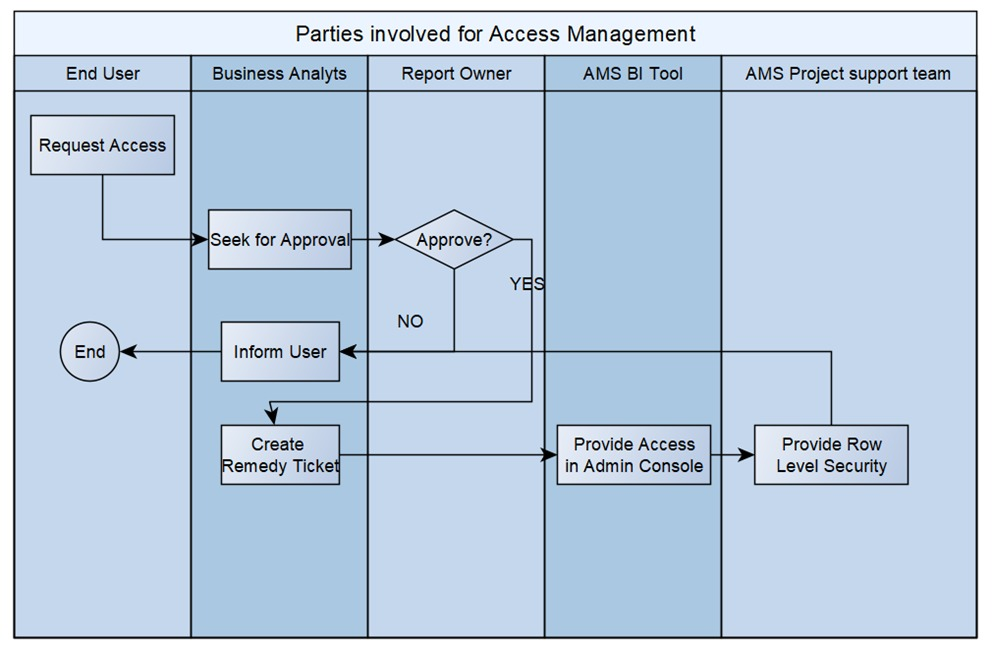
\includegraphics[width=15cm]{Workflow-aprobacion-original.jpeg}
%\caption{proceso Original}
\end{tabular}

El nuevo proceso resultante, quita del medio todos los elementos de "complejidad accidental", dejando simplemente a los únicos dos roles, que son relevantes, el "End User" que es el usuario final quien solicita el acceso al reporte y el "Report Owner" que es quien determina si la solicitud corresponde o no y puede actuar en consecuencia.

EL proceso resultante de la simplificación e integración del portal conlas herramientas de visualización y también del RLS (en caso de ser necesario), se describe a continuación:

\begin{tabular}{l}
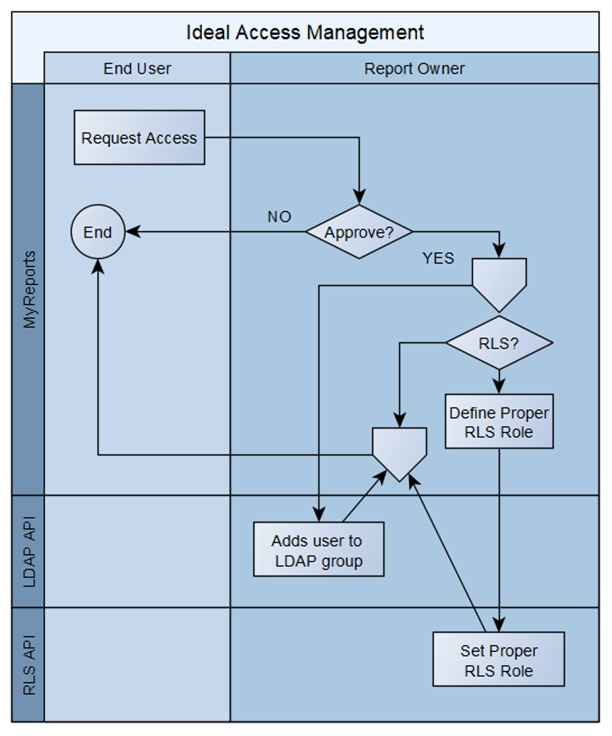
\includegraphics[width=10cm]{Workflow-aprobacion-mejorado.jpeg}
%\caption{Proceso simplificado}
\end{tabular}


\chapter{desarrollo y despliegue}
\section{Enfoque metodológico}

El proyecto se estructuró de modo clásico \gls{sdlc} con las siguientes fases:

\begin{enumerate}
    \item Ideación: del concepto y problema general a resolver.
    \item Especificación de requerimientos: Definicion de los requerimientos funcionales y no funcionales, junto con los criterios de aceptación.
    \item Diseño de la solución: Definición de la arquitectura, de los componentes logicos, del modelo de datos y de la experiencia de usuario (mediante maquetas).
    \item Desarrollo y pruebas: Fase de codificación y verificación de que el código cumple con los requerimientos y alcanza satisfactoriamente los criterios de aceptación.
    \item Despliegue a producción y lanzamiento: Fase de despliegue en el entorno productivo y tareas de capacitación y entrenamiento de usuarios (y de equipo de soporte/operaciones)
    \item Operación: fase en la que ya estando el sistema productivo, se le da soporte a los usuarios frente a incidentes.
    \item Decomisado: fase en la que se planifica y ejecuta el decomisado de la aplicación una vez que ya ha cumplido su ciclo de vida (todavía no ha ocurrido esto, ni se espera que ocurra en los proximos 2-3 años)
\end{enumerate}

%Cada fase estando muy bien definida con documentación formal como parte de los entregables de cada fase.

Inicialmente se decidió trabajar con una metodología \emph{Waterfall}, para poder enfocarse en un primer entregable, que pudiera cumplir con la funcionalidad básica de los casos de uso.


Para encarar el desarrollo, también se ensambló un equipo compuesto por los siguientes roles:

\begin{enumerate}
    \item Product Owner: Persona encargada de definir el producto, su roadmap, prioridades y fases de entregas para maximizar el valor de cada entrega, en múltiples fases de desarrollo.
    \item Project Manager: Persona encargada de armar el plan de trabajo con el product owner, los equipos de desarrollo, pruebas, operaciones y entrenamiento, para poder planificar las entregas y luego hacer la coordinar la ejecución y su seguimiento.
    \item Equipo de desarrollo: Equipo responsable por escribir el código y realizar pruebas unitarias y verificaciones iniciales del código. Conformado por programadores especializados en visualización, en logica de negocio y bases de datos. También hubo apoyo part time de un arquitecto para poder trabajar las definiciones estructurales y detalles de arquitectura definidas en la sección anterior.
    \item Equipo de testing: conformado por un líder de testing encargado de desarrollar los planes de pruebas, y desarrollar los casos de pruebas en funcion de las especificaciones de los casos de uso. Testers, encargados de ejecutar los casos de prueba, de distintos tipos, desde pruebas de integración, como así también de regresión y de performance.
    \item Equipo de operaciones: Este equipo es el responsable de operar el sistema una vez desplegado en producción y a la vez de dar continuidad a la operación, en caso de que alguno de los componentes falle por algún problema. Frente alguna situación de falla o reportes de errores de usuario, son la primer capa de atención al usuario y que permite analizar el síntoma y hacer un diagnóstico, para saber si lo reportado por los usuarios es realmente un error del sistema, un problema de experiencia de usuario o de entrenamiento.
    \item Equipo de capacitación: Equipo responsable de generar el material didáctico y planificar junto con el PM las capacitaciones de los usuarios, para poder garantizar una adopción adecuada del producto. También se explica el esquema de soporte en caso de necesitar reportar incidentes.
\end{enumerate}

\newpage
El esquema de trabajo en función de responsabilidades puede resumirse en la siguiente matriz \gls{raci}


\begin{figure}
\begin{tabular}{lcccccc}
\toprule
\textbf{Rol / Fase} & \textbf{Ideación} & \textbf{Reqs} & \textbf{Diseño} & \textbf{Desarrollo } & \textbf{Despliegue} & \textbf{Operación} \\
\midrule
PO & \textbf{A / R} & \textbf{A / R} & C & C & C & I \\
PM & C & C & \textbf{R} & A & \textbf{A / R} & I \\
Architect & C & C & \textbf{A} & R & C & I \\
Desarrollo & I & C & R / C & \textbf{R} & C & I \\
Testing & I & C & C & \textbf{R / C} & C & I \\
Operaciones & I & I & C & I & \textbf{I} & \textbf{R / A} \\
Capacitación & I & A & I & I & \textbf{R} & C \\
\bottomrule
\end{tabular}
    \caption{Matriz \gls{raci}-\gls{sdlc} para el equipo definido}
    \label{fig:raci_matrix} 
\end{figure}

    \newpage

\begin{figure}
\begin{tikzpicture}[
  role/.style={rectangle, draw, rounded corners, align=center, minimum height=1.5cm},
  arr/.style={-{Stealth}, thick}
  ]

  % Nodos
  \coordinate (anchoro) at (-5cm,0cm);
  \node[role, right=10cm of anchoro] (PO) {Product Owner};
  \node[role, below=of PO] (PM) {Project Manager};
  \node[role, below=of PM] (DEV) {Equipo de Desarrollo};
  \node[role, right=of DEV] (TEST) {Equipo de Testing};
  \node[role, below=of TEST] (OPS) {Equipo de Operaciones};
  \node[role, right=of TEST] (TRAIN) {Equipo de Capacitación};

  % Flechas principales
  \draw[arr] (PO) -- (PM);
  \draw[arr] (PM) -- (DEV);
  \draw[arr] (PM) -- (TEST);
  \draw[arr] (PM) -- (OPS);
  \draw[arr] (PM) -- (TRAIN);

  % Interacciones entre equipos
  \draw[arr] (DEV) -- (TEST);
  \draw[arr] (TEST) -- (DEV);
  \draw[arr] (DEV) -- (OPS);
  \draw[arr] (OPS) -- (DEV);

  \draw[arr] (TRAIN) -- (DEV);
  \draw[arr] (TRAIN) -- (OPS);
  \draw[arr] (TRAIN) -- (PM);

\end{tikzpicture}
    \caption{Interacciones entre roles/sub-equipos}
    \label{fig:ways_of_working} 
\end{figure}


En esta metodología de desarrollo waterfall, se encuentran diferentes entornos de trabajo, dedicados a distintos fines y a la vez, a los que se accede, al cumplir satisfactoriamente diferentes verificaciones del ciclo de desarrollo.

\begin{tabular}{l}
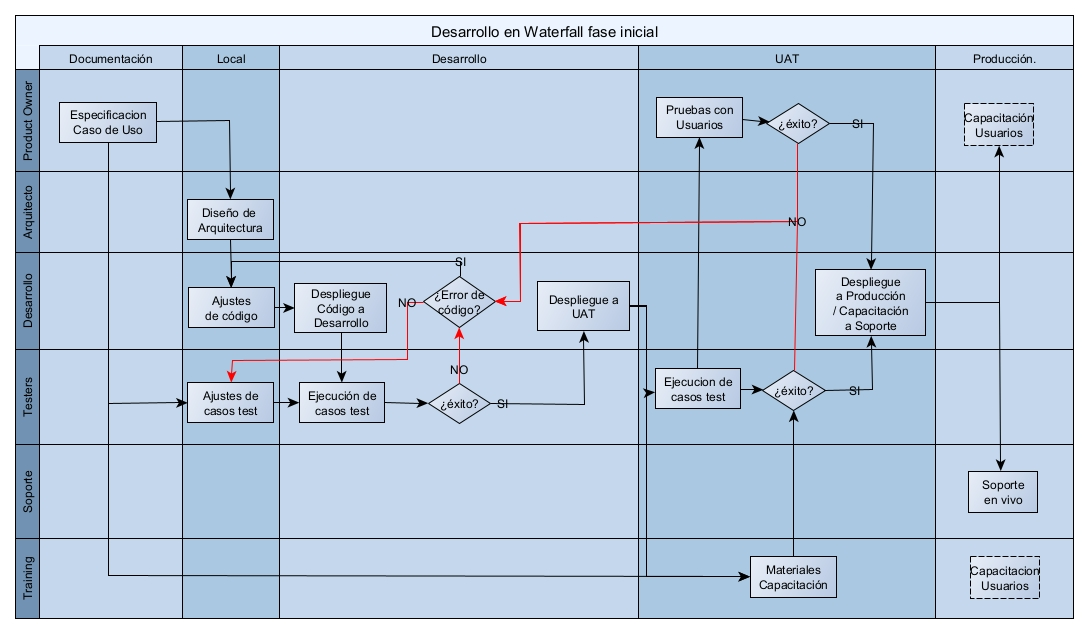
\includegraphics[width=15cm]{waterfal_dev_phase1.jpg}
%\caption{Actividades según roles y entornos}
\end{tabular}

\begin{enumerate}
    \item Entornos locales: En los entornos locales, se trabaja de manera independiente en la documentación de casos de uso, diseño de arquitectura y luego cada desarrollador y tester, trabaja con versiones locales del codigo. En este caso, pueden exisistir múltiples versiones del mismo código que se modifican en paralelo por los distintos desarrolladores, según se hayan dividido las tareas según los skills de los miembros del equipo. (puede ser front end, back end, modelos de datos, apis, etc.).

        A su vez, el equipo de testing, en sus equipos locales, también desarrolla sus casos de prueba, alineados con la funcionalidad definida en la especificación, pero sin interactuar con el equipo de desarrollo, de modo que se toma como base la especifiación y no el código que desarrollan los programadores. De este modo, el equipo de testing se enfoca 100\% en la escencia de la funcionalidad y no necesariamente en cómo se ha desarrollado/implementado la funcionalidad.
    
    
    \item Entorno de Dev: En el entorno de Dev. (o de Desarrollo), es el primero entorno en el que se realizan pruebas del código generado por los multiples desarrolladores, ya combinado en una versión candidata para ser lanzada a producción. Es el espacio donde el equipo de testing puede correr la totalidad de los casos de pruebas que generaron y se evalúan los resultados de las ejecuciones. Si son exitosas, en principio se habilita esa versión de la aplicación/código para ser promovido al entorno de UAT.
    
    En caso de resultar fallidas, el equipo de testing trabaja junto con el equipo de desarrollo para hacer el troubleshooting de aquellos casos fallidos y en función de los hallazgos:
        \begin{enumerate}
            \item se corrije el código porque tenía defectos.
            \item se corrije caso de test porque tenía defectos.
            \item se corrijen el código y el caso de test porque ambos tenían defectos.
        \end{enumerate}
    
    Finalmente, se vuelve a unificar el código y los casos de pruebas ajustados para luego repetir las pruebas en el entorno de desarrollo hasta que todo sea satisfactorio.

    \item Entorno de UAT: Este es el entorno donde el Product Owner, habilita acceso a ciertos usuarios clave, que ayudan a hacer una verificación del sistema para dar el visto bueno para poder pasar el sistema a producción. De surgir fallas, se reportan al equipo de testing y de desarrollo y se realiza el troubleshooting de modo similar al del estadio anterior. De este modo, cualquier falla que se detecta, lleva el proceso al ajuste de código y luego a las pruebas en el estadio anterior.
    
        Una vez que la aplicación se ha desplegado al entorno de UAT, las interfaces de usuario ya son práctiamente definitivas y el equipo de capacitación puede trabajar en el desarrollo de los materiales para la capacitación de los usuarios finales.
    
    \item Entorno de Producción: Una vez que las pruebas en el entorno de UAT han sido superadas con éxito, se hace el pasaje final a producción y ocurren dos actividades escenciales. El product owner queda ya habilitado para comenzar las sesiones de capacitación según el plan de despliegue y entrenamiento y el equipo de desarrollo realiza una transferencia de conocimiento y capacitación (junto con la entrega de la documentación correspondiente) para que el equpo de operaciones, comience a dar el soporte necesario con la plataforma ya en vivo. 
    
    El product owner, junto con el equipo de capacitación (training) hacen el lanzamiento y las campañas de comuniación/entrenamiento con la finalidad de entrenar a los usuarios en el uso del sistema y luego trabajar en la adopción del mismo.
\end{enumerate}

\section{Estrategia de despliegue y fases de rollout.}

Para la estrategia de despliege, se optó, por un enfoque en dos fases. una Fase I, que consistía en un \gls{mvp} con un pequeño grupo piloto de colaboración cercana, de modo de tener un primer acercamiento al uso real del sistema, con quienes se pudo trabajar muy de cerca. Esto permitió que se puedan testear las hipótesis y recolectar feedback valioso, para poder refinar los casos de uso originales.

Luego, se pasó a la fase II, fomentando un crecimiento "orgánico", donde se identificaron equipos clave en el resto de la organización y se fueron sumando gradualmente en un período de 12 meses.

\subsection{Fase I: \gls{mvp} con Grupo piloto}
    
Para hacer el despliegue, se realizó la puesta en producción y se seleccionó un equipo de usuarios que trabajaba con la región de latinoamérica. Ellos tenían muy buena formación técnica y eran los clientes indicados para poder dar el puntapié inicial al despliegue global.

Se trabajó entonces con este equipo en modo piloto inicial y los resultados fueron alentadores. 

Se realizaron las capacitaciones y luego estableció un período de tres meses para dejar rodar la solución y a la vez evaluar la estabilidad, performance y mejorar temas necesarios que no habían sido considerados como para poder luego hacer el rollout global.

\subsection{Fase II: Expansión y escalamiento a más áreas y usuarios}

Ya con el piloto satisfactorio, una lista mínima de mejoras ya implementadas y el equipo redefinido junto con la metodología, se decidió expandir el piloto al resto de las regiones y otros equipos corporativos. El despliege completo duró aproxiamdamente 6 meses más y a medida que se fue avanzando cada vez se fue simplificando más el proceso de "onboarding" de nuevos usuarios.

Se adoptó un enfoque de entrenamiento para los creadores de contenidos y ellos a su vez comenzaron a promocionarlo y entrenar a sus propios usuarios y en muchos casos, cuando había usuarios que ya usaban el portal por otros creadores de contenido, preguntaban proactivamente por qué faltaban agregar más contenidos, con lo cual el crecimiento se dio de modo orgánico y natural.

\section{Plan de comunicación y capacitación}
El plan de comunicación y de capacitación, se diseñó de modo de acompañar las fases de despliegue por grupos de usuarios y audiencias. Se encaró un enfoque de \gls{cop}, que permitió crear un universo de usuarios general, con algunos más "expertos" que ayudaron a disceminar las mejores prácticas. 

se identificaron dichos usuarios líderes o clave y se hizo una capacitación del estilo \gls{ttt}, para poder hacerlo en múltiples olas y a la vez de modo federado y escalable.

Los materiales de soporte y guías de usuario, se defineron en dos niveles: 
\begin{enumerate}
    \item Guía específica para usuarios con privilegios de publicación y administración de contenidos
    \item Guía para usuarios finales, que en realidad estaba integrada al portal, e incluso la misma interfaz era bastante auto descriptiva.
\end{enumerate}

\section{Mecanismos de soporte post-lanzamiento}

Dentro del esquema de soporte, se trabajó con un equipo corporativo que maneja un esquema de soporte de dos niveles. El primer nivel, orientado a preguntas simples y que son de solucion fácil, como pueden ser problemas de conectividad, instrucciones básicas sobre el uso del portal o eventualmente sobre alguno de los reportes. Si el primer nivel, no puede resolver satisfactoriamente la consulta del usuario, entonces se derivaba a un segundo nivel donde se identificaba, según la naturaleza de la consulta, qué acción seguir y qué grupo debía darle seguimiento.

Es importante destacar que el objetivo del equipo de nivel 2, es garantizar la continuidad del servicio y mantener el sistema disponible y los accesos de los usuarios activados.

En caso de que los usuarios finales hayan reportado un comportamiento compatible con un defecto o bug, entonces se derivaba al equipo de desarrollo para seguir con máxima prioridad un proceso de troubleshooting y análisis de causa raíz, para a su vez aplicar una solución definitiva.


\section{Gestión de calidad y ajustes/mejoras metodológicas}


Inicialmente, la calidad del desarrollo se fue monitoreando mediante el equipo de testing. EL leader de testing había creado un plan de pruebas y estas pruebas eran ejecutadas y documentadas rigurosamente antes de realizar pasajes a producción. 


En caso de encontrar errores, se notificaban registraban en una plataforma que utilizabamos para tal fin y se compartían con el equipo de desarrollo y luego de corregirse, se re-verificaban. 


El proceso era muy manual y no permitía, ni gran agilidad, ni múltiples y rápidas iteraciones a la hora de lanzar nuevas versiones a producción.


Después de un período inicial de desarrollo de 6 meses, se logró alcanzar el primer hito, donde se implementaron de manera básica todos los casos de uso definidos inicialmente. 


Esto por un lado permitió ofrecer un MVP útil y funcional y a la vez, detectar oportunidades de mejora y evoluciones posibles, ya con el sistema rodando en el entorno de producción.


Para poder encarar sucesivas iteraciones en la evolución de la plataforma, se tuvo que cambiar drásticamente la composición del equipo, como así también la metodología de desarrollo, de modo tal de poder responder on mayor agilidad a los cambios y necesidades aumentando significativamente calidad y reduciendo los plazos de entrega.


Los cambios, fueron sustantivos y afectaron, no sólo la metodología de desarrollo, sino también la composición del equipo de desarrollo y operaciones.


Las principales causas para revisar la forma de trabajo fueron las siguientes:
El esfuerzo manual de testeo, por parte del equipo de testing era excesivo, lento y un verdadero cuello de botella. La forma en la que se documentaban los defectos, a veces era inconsistente y se podían duplicar y a medida que la complejidad de la aplicación aumentaba, los casos de pruebas y sus tiempos de ejecución crecían de modo exponencial. La complejidad y diversidad casuística aumentaba a un ritmo mucho mayor que el código que la soportaba y era fundamental buscar alternativas.


Esto además tenía un impacto muy negativo en los ciclos de entrega, haciendonos demorar meses hasta que una versión inicial y funcional, llegó a un punto de madurez que la hizo "usable".


Adicionalmente, había problemas en la calidad del código desarrollado por los desarrolladores, porque al demorarse las entregas, la presión por terminar aumentaba e impactaba los entregables generando retrabajo. 


Finalmente, cuando llegaban las versiones al entorno de producción, notamos que en varias ocasiones, a pesar de haber pasado satisfactoriamente las fases de testeo y control de calidad, tenían defectos y el equipo de operaciones, tampoco era efectivo a la hora de resolver algunos incidentes, por falta de conocimiento de la aplicación, y las capacitaciones que el equipo de desarrollo les daba al hacer los despliegues productivos, eran complejas o insuficientes.

\begin{table} 
    \centering
    \begin{tabular}{|c|c|c|c|}\hline
        \textbf{Actividades}&  \textbf{Waterfall}&  \textbf{DevOps Interino}&  \textbf{DevOps Final}\\\hline
         Esquema de entregas&  1 x Trimestre &  1 x Mes & 1-3 x Semana  \\\hline
         Cobertura del código& $\approx 25$\% &  $\approx 25$\%&  $\approx 50$\%\\\hline
         Pruebas de Regresión (hs)&  24&  1&  2\\\hline
         Tiempos de Hand Over (hs)& 8&  4&  -\\\hline
         Tasa de defectos desde Prod\\ (vs trabajo nuevo x mes)&  $\approx 30$\%&  $\approx 15$\%&  $\approx 5$\%\\\hline
    \end{tabular}
    \caption{Mejoras metodológicas}
    \label{tab:water_to_devops_method}
\end{table}

A continuación, se detalla cómo ha evolucionado la composición del equipo, a medida que se avanzó con la transformación metodológica, comparando \gls{fte}.

\begin{table}
    \centering
    \begin{tabular}{|c|c|c|c|}\hline
        \textbf{Composición del Equipo}&  \textbf{Waterfall}&  \textbf{DevOps Interino}&  \textbf{DevOps Final}\\\hline
         ProductOwner&  1 &  1 & 1  \\\hline
         PM/ScrumMaster& 1 &  1&  1\\\hline
         Desarroladores&  4&  4&  4\\\hline
         Arquitecto& 0,3&  0,3&  0,3\\\hline
         DevOps Engineer& 0&  0,1&  0,1\\\hline
         Lead de Test& 1&  1&  0\\\hline
         Testers& 4&  3&  0\\\hline
         Testers+& 0&  2&  2\\\hline
         Training& 0,3&  0,3&  0,3\\\hline
         Support Lead& 1&  0&  0\\\hline
         Support& 1&  0&  0\\\hline
         Total & 13,9&  13,4&  8,4\\\hline         
         Evolucion s\% & 100\%& $\approx 96$ \% &  $\approx 60$\%\\\hline         
        \end{tabular}
    \caption{Evolución del Equipo}
    \label{tab:water_to_devops_team}
\end{table}

\chapter{evaluacion}
\section{Metodología de evaluación}
\section{Resultados cuantitativos}
\section{Resultados cualitativos}
\section{Comparación con KPIs iniciales}
\section{Impacto en seguridad y cumplimiento}
\section{Conclusiones de la evaluación}
\chapter{Conclusiones}
\section{Resumen de los logros principales}
\section{Relevancia del proyecto para la organización}
\section{Impacto estratégico a largo plazo}
\section{Próximos pasos sugeridos (roadmap evolutivo)}

\chapter{Lecciones Aprendidas}

\section{Aspectos que funcionaron bien}
\section{Dificultades y cómo se superaron}
\section{Factores clave de éxito}
\section{Aspectos a mejorar}
\section{Aprendizajes organizacionales}
\section{Recomendaciones para futuros proyectos}


%% ...

%%%% BIBLIOGRAFIA
\backmatter
%\bibliography{tesis}
\printbibliography
\printglossary



\end{document}
